\renewcommand{\arraystretch}{0.1}% Tighter
\centering \footnotesize
\begin{tikzpicture}
\node[] (start) {};
\node[left=1cm of start] (sfsigma) {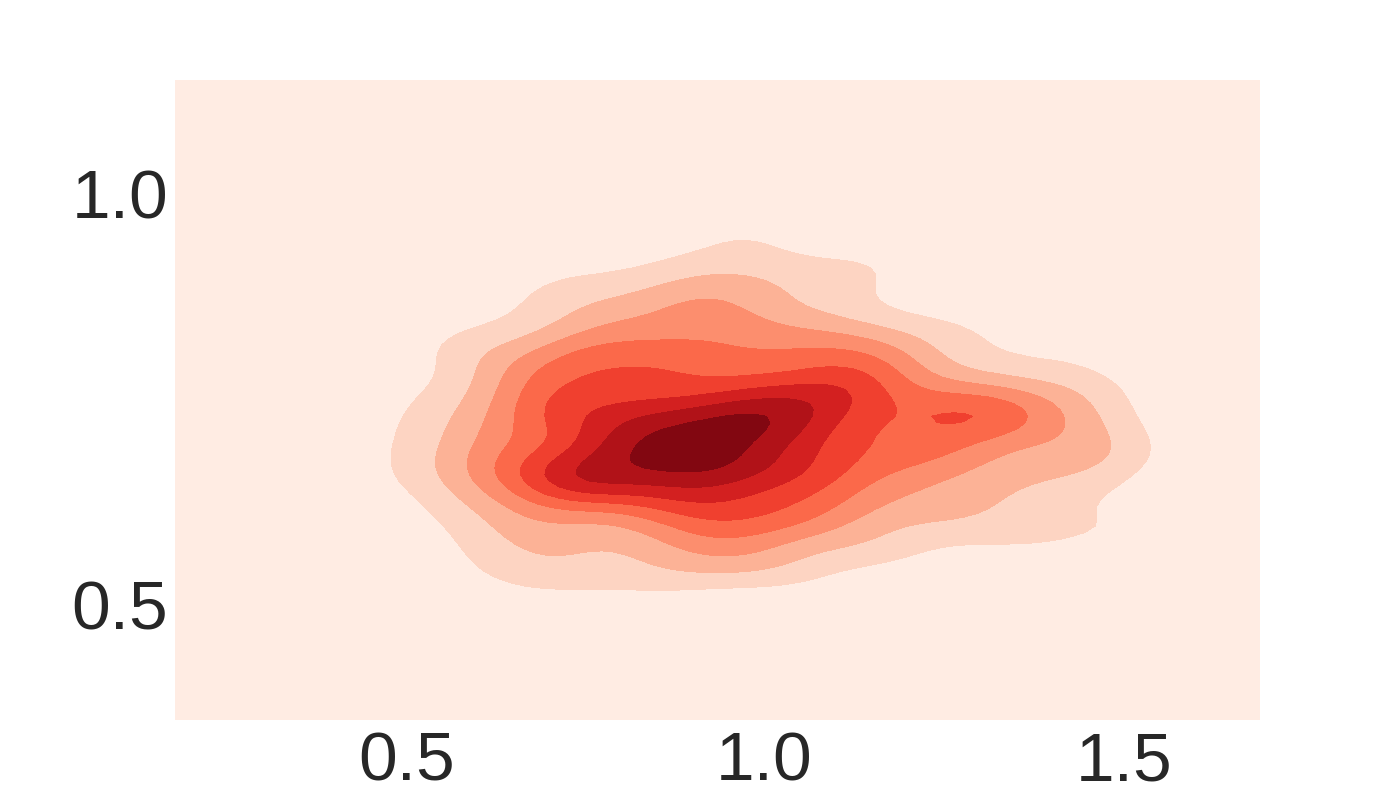
\includegraphics[height=2cm]{figs/hypers_sf_sigma.png}};
\node[right=1cm of start] (sfell) {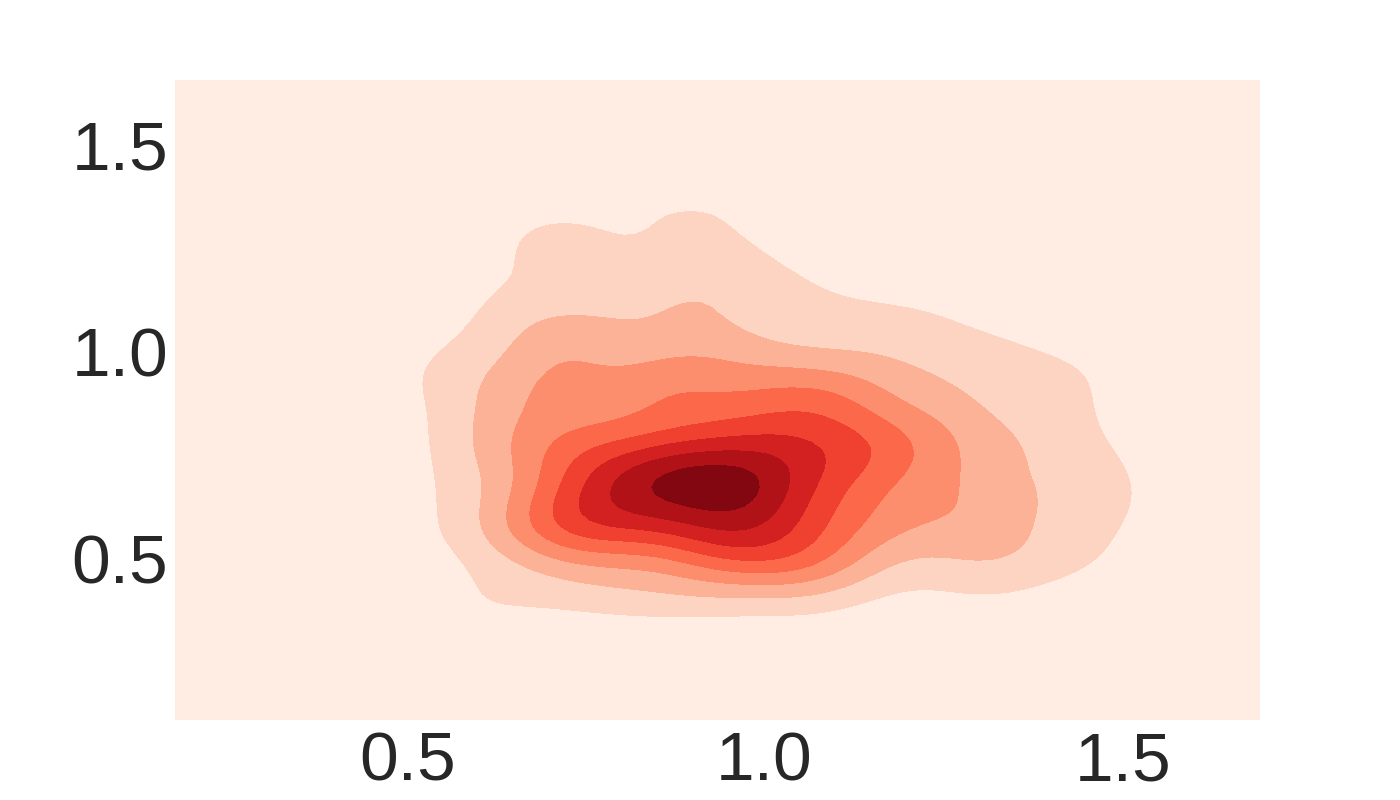
\includegraphics[height=2cm]{figs/hypers_sf_ell.png}};
\node[above=1cm of start] (hyper) {(a) $P(\bm{\theta} = \{\ell,sf,\sigma\} \mid
\mathbf{D},\Krv)$};
\node[left=0.cm of sfsigma] (ell) {$\ell$};
\node[below=0.cm of sfsigma] (sf1) {$sf$};
\node[left=0.cm of sfell] (sigma) {$\sigma$};
\node[below=0.cm of sfell] (sf2) {$sf$};






%%%%%%%%%%%%%%%%%%%%%%%%%%%%%%%%%%%%%%%%%%%%%%%%%%%%%%%%%%%%
%%%%%%%%%%%%  Code             %%%%%%%%%%%%%%%%%%%%%%%%%%%%%
%%%%%%%%%%%%%%%%%%%%%%%%%%%%%%%%%%%%%%%%%%%%%%%%%%%%%%%%%%%%

\node[below=1.0cm of start] (b_code){
\footnotesize\begin{lstlisting}[mathescape,escapechar=\#]
// Define data and look-up function
define data = array(array(-1.87, 0.13), ..., array(1.67, 0.81));
assume f_look_up = proc(index) {lookup(data, index)};
\end{lstlisting}
};
\node[below=-0.65cm of b_code,xshift=-0.58cm] (c_code){
\footnotesize\begin{lstlisting}[mathescape,escapechar=\#
]
// Initialize hyper-priors
assume alpha_sf = tag(scope="hyperhyper", gamma(5,1));
assume beta_sf  = tag(scope="hyperhyper", gamma(5,1));
assume alpha_l  = tag(scope="hyperhyper", gamma(5,1));
assume beta_l   = tag(scope="hyperhyper", gamma(5,1));#\vspace{1mm}#
assume sf = tag(scope="hyper", gamma(alpha_sf, beta_sf)));
assume l  = tag(scope="hyper", gamma(alpha_l, beta_l)));
\end{lstlisting}
};
% (d) & (e)
\node[below=-0.72cm of c_code,xshift=-0.65cm] (d_code){
\footnotesize\begin{lstlisting}[mathescape,escapechar=\#]
// Initialize covariance function
assume se = apply_function(make_squaredexp(sf, l));
assume wn = apply_function(make_whitenoise(sigma));
assume composite_covariance = add_funcs(se, wn);#\vspace{8mm}#
// Create a prober and emulator using gpmem
assume (f_compute, f_emu) =
    gpmem(f_look_up, composite_covariance);#\vspace{1mm}#
sample f_emu(array(-2, $\cdots$, 2));
\end{lstlisting}
};
% (f)
\node[below=0.01cm of d_code,xshift=-0.18cm] (e_code){
\footnotesize\begin{lstlisting}[mathescape,escapechar=\#]
// Observe all data points
for (n = 0; n < size(data); n++){
    observe f_emu(first(lookup(data,n))) =
        second(lookup(data,n))};
// Or: probe all data points
for (n = 0; n < size(data); n++){
    predict f_compute(first(lookup(data,n)))};#\vspace{1mm}#
sample f_emu(array(-2, $\cdots$, 2));
\end{lstlisting}
};
% (g)
\node[below=-0.0cm of e_code,xshift=-0.77cm] (f_code){
\footnotesize\begin{lstlisting}[mathescape,escapechar=\#]
// Metropolis-Hastings
infer repeat(100, do(
    mh(scope="hyperhyper", steps=1),
    mh(scope="hyper",      steps=3)));#\vspace{1mm}#
sample f_emu(array(-2, $\cdots$, 2));
\end{lstlisting}
};

\node[below=0.5cm of f_code,xshift=0.3cm] (g_code){
\footnotesize\begin{lstlisting}[mathescape,escapechar=\#]
// Optimization
infer gradient-ascent(scope="hyper",
			       steps=10);

sample f_emu(array(-2, $\cdots$, 2));
\end{lstlisting}
};



% samples/curve images
\node[below=1.2cm of c_code,xshift=6cm] (d_pic){
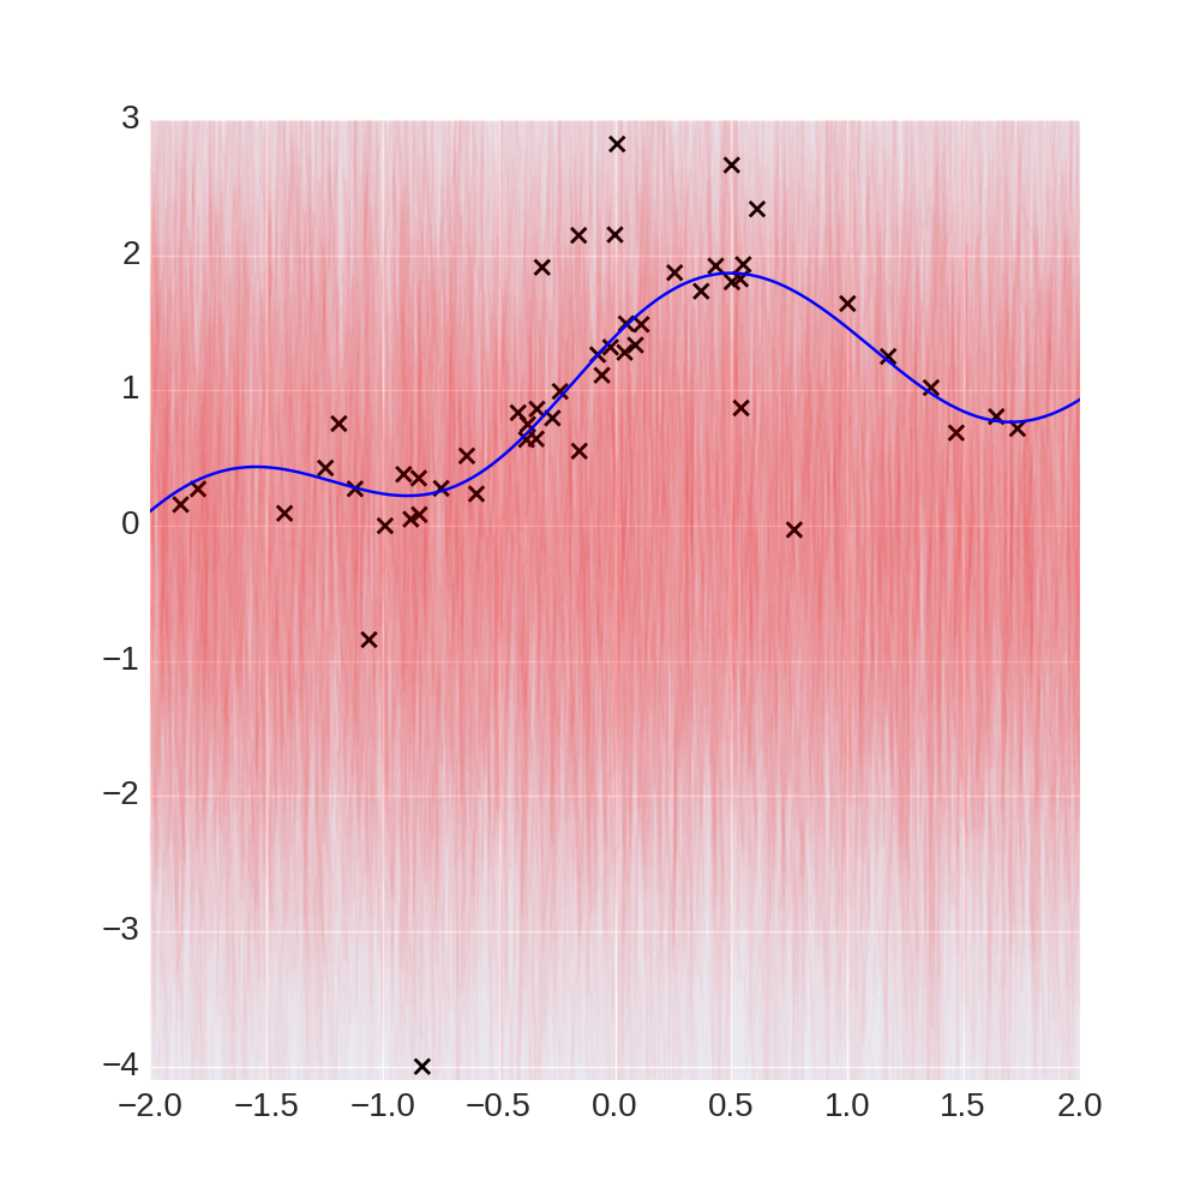
\includegraphics[height=3.4cm]{figs/neal_example_before_observation.jpg}
};
\node[below=-0.4cm of d_pic] (e_pic){
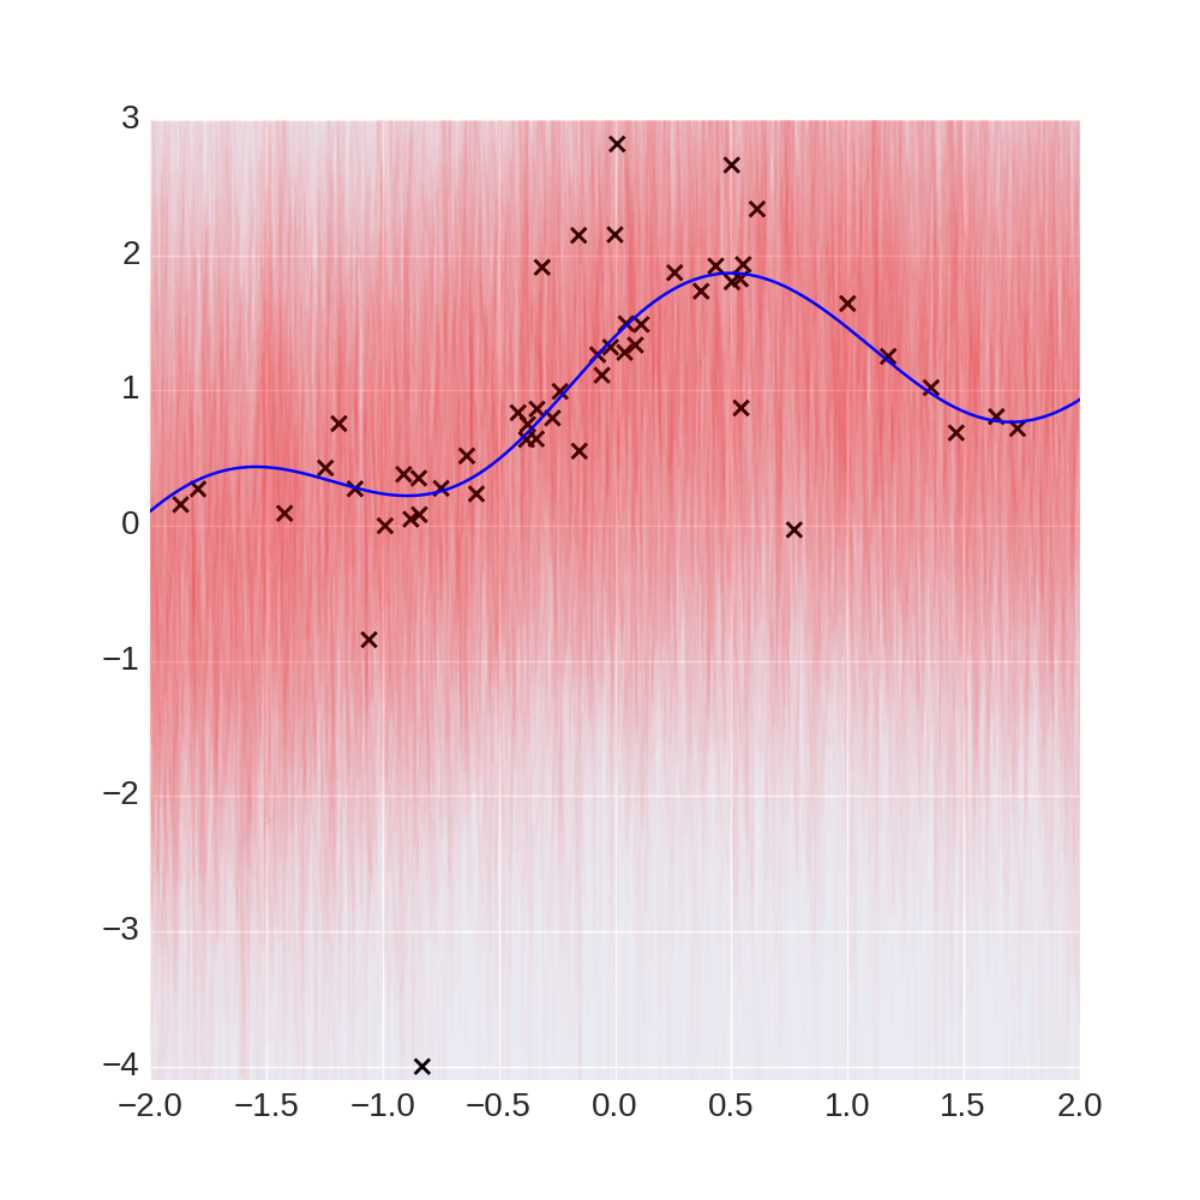
\includegraphics[height=3.4cm]{figs/neal_example_after_observation.jpg}
};
\node[below=-0.4cm of e_pic] (f_pic){
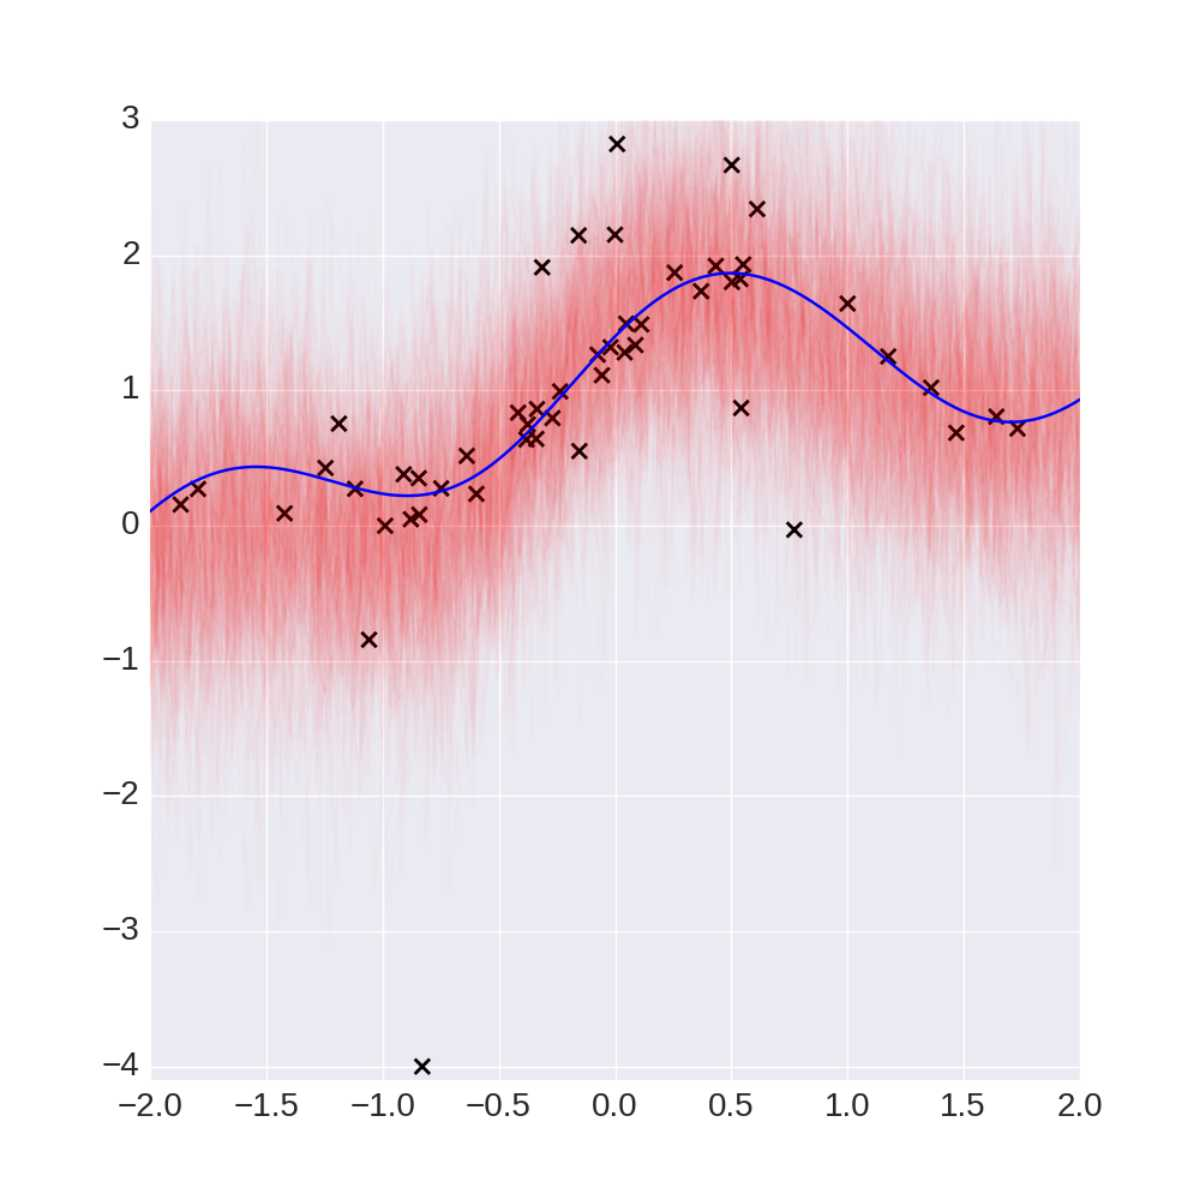
\includegraphics[height=3.4cm]{figs/neal_Bayesian.jpg}
};
\node[below=-0.4cm of f_pic] (g_pic){
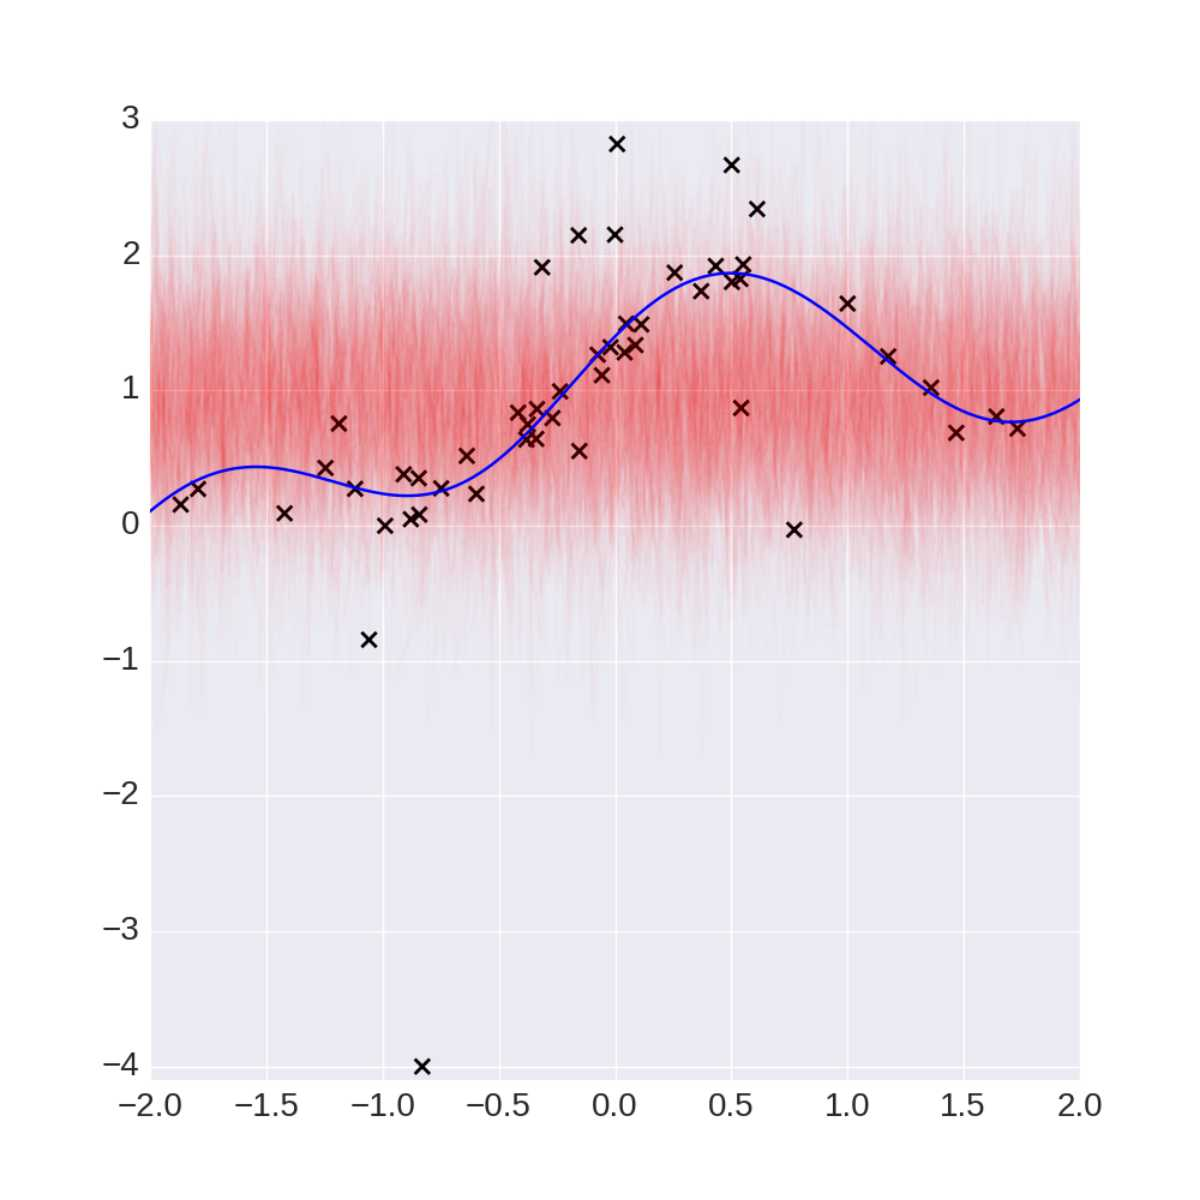
\includegraphics[height=3.4cm]{figs/neal_example_map_inference_alpha0p01_iter15.jpg}
};

% horizontal lines
% (a)
\draw 
  ([xshift=-0.2cm,yshift=-0.6cm]b_code.north west) --
([xshift=0.8cm,yshift=-0.6cm]b_code.north east); 
% (b)
\draw 
  ([xshift=-0.2cm,yshift=0.08cm]b_code.south west) -- ([xshift=0.8cm,yshift=0.08cm]b_code.south east);   
% (c)
 \draw 
  ([xshift=-0.2cm,yshift=-2.75cm]b_code.south west) --
([xshift=0.8cm,yshift=-2.75cm]b_code.south east); 
% (d)
 \draw 
  ([xshift=-0.2cm,yshift=-4.45cm]b_code.south west) --
([xshift=0.8cm,yshift=-4.45cm]b_code.south east); 
% (e)
 \draw 
  ([xshift=-0.2cm,yshift=-7.5cm]b_code.south west) -- ([xshift=0.8cm,yshift=-7.5cm]b_code.south east); 
% (f)
 \draw 
  ([xshift=-0.2cm,yshift=-10.8cm]b_code.south west) -- ([xshift=0.8cm,yshift=-10.8cm]b_code.south east); 
% (g)
 \draw 
  ([xshift=-0.2cm,yshift=-14.1cm]b_code.south west) -- ([xshift=0.8cm,yshift=-14.1cm]b_code.south east); 

% labels
\node[below=1.9cm of start,xshift=-6.5cm] (b) {(b)};
\node[below=1.4cm of b] (c) {(c)};
\node[below=1.9cm of c] (d) {(d)};
\node[below=1.7cm of d] (e) {(e)};
\node[below=2.6cm of e] (f) {(f)};
\node[below=2.9cm of f] (g) {(g)};
\node[below=2.6cm of g] (h) {(h)};
\end{tikzpicture}

